\setcounter{secnumdepth}{3} %para tener una profundidad más en las enumeraciones
\chapter{Evaluacion Con Usuarios}
\label{cap:evaluacionConUsuarios}
Tras las fases de desarrollo de la herramienta se llevarán a cabo las pruebas con usuarios que nos mostrarán los datos de un primer contacto con usuarios.\\
Para eso hemos creado un guión de evaluación que fijará unos objetivos y unas preguntas de investigación, así como marcar las pautas para la realización de las pruebas. \\
Después de la realización de las pruebas se procederá a hacer una análisis que muestre las posibles brechas encontradas, basándonos en la experiencia de los usuarios. \\

\section{Objetivos y preguntas de investigación} \label{sec:preguntas}
Los objetivos y preguntas de investigación tienen como finalidad tratar de comprender la experiencia de los usuarios reales al interactuar con nuestra herramienta por primera vez. Buscamos identificar cualquier punto donde puedan surgir dificultades, confusión o áreas donde la herramienta podría ser más efectiva. Para guiar esta exploración, hemos definido los siguientes objetivos y preguntas de investigación.

\subsection{¿Resulta intuitiva y clara la herramienta para el usuario?} \label{sec:intuitiva}
Lo más importante de la herramienta es que sea clara para los usuarios que van a usarla, ya que sin eso, aunque la herramienta tenga un buen funcionamiento, la utilidad de esta sigue siendo nula.\\
Nuestro primer objetivo se centra en evaluar si los usuarios perciben la interfaz y los flujos de trabajo de manera natural y sin ambigüedades.\\

Preguntas de investigación relacionadas con el objetivo:
\subsubsection{¿El usuario entiende fácilmente cómo añadir funcionalidad al enemigo?}
Esta pregunta de investigación pretende comprobar, si el usuario es capaz de comprender el funcionamiento base de los enemigos, es decir, si comprende como utilizar la máquina de estados o como se añaden estados nuevos, transiciones, Damage Emitters y actuadores.\\

\subsubsection{¿Las opciones de comportamiento ofrecidas son comprendidas en su totalidad?}
Aquí, nuestro interés reside en la claridad con la que se presentan y se entienden los distintos actuadores disponibles. Buscamos identificar cualquier punto de confusión en su aplicación, analizando si la funcionalidad y las explicaciones proporcionadas para cada uno son suficientes para su correcta utilización.\\

\subsubsection{¿La interfaz comunica correctamente el propósito de cada estado y transición?}
La pregunta de investigación pretende conocer si el diseñador es capaz de saber en todo momento en que estado está el enemigo y por tanto que comportamiento cabría esperar.\\

\subsubsection{¿La documentación aclara y detalla la configuración de las funcionalidades?}
Buscamos evaluar si la documentación adjunta proporciona la información necesaria para que el usuario pueda configurar correctamente los enemigos, aprovechando al máximo las funcionalidades implementadas. \\

\subsection{¿El sistema de creación de enemigos demuestra ser funcional?}  \label{sec:funcional}
Este objetivo busca validar la operatividad y la utilidad de la herramienta.\\

Preguntas de investigación relacionadas con el objetivo:
\subsubsection{¿La herramienta agiliza y simplifica el proceso de diseño de enemigos?}
Esta pregunta se enfoca en la eficiencia que aporta la herramienta al flujo de trabajo del diseñador de videojuegos. ¿Facilita la creación de enemigos?\\

\subsubsection{¿El comportamiento de los enemigos generados se corresponde con lo esperado en el videojuego?}
En este punto, la atención se centra en la fidelidad con la que la lógica definida en la herramienta se manifiesta en el entorno de juego. ¿Actúan los enemigos según lo previsto? ¿Se activan sus acciones en las circunstancias correctas? Identificar cualquier desviación entre el diseño y la ejecución es crucial.\\

\subsubsection{¿La herramienta permite la adaptación y expansión sencilla de los enemigos?}
Queremos evaluar si es posible modificar o ampliar las capacidades de los enemigos creados mediante la adición de nuevos comportamientos o la alteración de parámetros existentes, sin generar complejidad innecesaria.

\section{Diseño de la Evaluación}
En esta sección se detalla la planificación y la estructura de las pruebas con usuarios.

\subsection{Audiencia Objetivo}
\begin{itemize}
\item Edad: mayor de 18 años
\item Genero: No relevante
\item Extracto Sociocultural: El público objetivo se centra en perfiles que tengan un extracto sociocultural relacionado con el diseño de videojuegos. Esto incluye:
\begin{itemize}
\item Estudiantes actuales o pasados de diseño de videojuegos.
\item Profesionales que se dediquen o tengan interés en la creación de enemigos.
\item Personas que sin poseer estudios específicos demuestren tener interés en la creación de entidades y sus comportamientos. 
\end{itemize}

\item Habilidades Requeridas:  Se espera que los participantes en la evaluación cuenten con conocimientos previos en diseño de personajes, conceptos básicos del funcionamiento de Unity y comprensión básica de maquinas de estado.
\end{itemize}

\subsection{Duración y Entorno de Realización}
Cada sesión de prueba se extenderá durante unos 60 minutos. Este lapso lo dedicaremos primero a una breve charla introductoria sobre la prueba. Luego, se pedirá que se explore el manual y realicen los ejemplos prácticos. Finalmente se realizará una entrevista que proporcionará feedback adicional.\\

Las sesiones se realizarán en entornos controlados y tranquilos donde el usuario no tenga distracciones. Se dispondrá un ordenador con la herramienta ya instalada y lista para su uso, así como teclado y ratón estándar. Al haber simultaneidad de pruebas con varios usuarios, para evitar la influencia entre ellos se procurará situarlos separados entre ellos y en caso de que no fuese posible, pedirles la mínima interacción posible entre ellos.

\subsection{Descripción de Tareas del Probador}
El probador deberá realizar las siguientes actividades:

\begin{itemize}
\item Lectura del manual (sin ejemplos de uso). Estimación: 10 minutos.
\item Ejecución de ejemplos de uso. Estimación: 30 minutos.
\item Creación libre de un enemigo. Estimación 10 minutos
\item Realización del cuestionario. Estimación 5 minutos.
\item Realización de la entrevista. Estimación 5 minutos.
\end{itemize}

Las tareas se presentarán de forma secuencial, permitiendo al usuario familiarizarse gradualmente con las funcionalidades de la herramienta. 

\subsection{Instrucciones Iniciales}

Antes de comenzar las pruebas se agradecerá la participación de los usuarios. Se dejará claro al inicio que no es una crítica hacia ellos y que solo estamos evaluando la funcionalidad de la herramienta y en ningún caso juzgándoles, además, se les indicará las diferentes partes que consta la evaluación.\\

Guion de la sesión:\\

"Buenos días a todos y muchísimas gracias por la colaboración en estas pruebas de evaluación.
Como ya sabéis, vais a probar una herramienta que sirve para diseñar enemigos en dos dimensiones en Unity.
En los ordenadores tenéis ya un proyecto con la herramienta abierta, así como un manual de usuario detallado en el escritorio.
Por favor leed el manual y haced los ejemplos prácticos que se describen dentro de él. Una vez familiarizados con la herramienta y habiendo terminado los ejemplos prácticos, usadla creando el enemigo que se os ocurra.
Por último se os abrirá un breve cuestionario, para su cumplimentación y terminaremos con una breve entrevista."

\subsection{Comportamiento del Investigador}

Durante toda la sesión de pruebas, el investigador actuará como observador imparcial y facilitador. Su presencia tendrá como objetivo principal garantizar que los participantes comprendan las instrucciones generales y ofrecer soporte logístico en caso de que surjan problemas técnicos o situaciones inesperadas. No se ofrecerá ayuda directa sobre el uso de la herramienta salvo que una situación impida completamente continuar con la evaluación, ya que se busca observar cómo los usuarios interactúan con la interfaz sin intervenciones externas.\\

El investigador evitará cualquier influencia en las decisiones o acciones del usuario, no corrigiendo ni orientando sobre cómo utilizar la herramienta. Anotará observaciones relevantes sobre el comportamiento del usuario, como expresiones de duda, errores recurrentes, pasos omitidos o dificultades generales en la navegación.\\

Al finalizar la sesión, el investigador facilitará la entrevista, siguiendo una estructura abierta pero guiada que permita profundizar en las impresiones subjetivas de cada usuario.\\

\subsection{Metodología}

La evaluación ha sido diseñada utilizando una metodología mixta, combinando técnicas cuantitativas y cualitativas para obtener una visión completa del desempeño de la herramienta.
\subsubsection{Observación}
Durante la realización de las tareas, el investigador observará el comportamiento de los participantes de forma no intrusiva. Se tomarán notas sobre:

\begin{itemize}
\item Dudas frecuentes o repetitivas.
\item Tiempos estimados de realización por tarea.
\item Momentos de frustración, vacilación o errores.
\item Fluidez general en la interacción con la interfaz.
\end{itemize}
Esta observación permitirá identificar posibles problemas de usabilidad no detectados únicamente a través del cuestionario o la entrevista.

\subsubsection{Cuestionario}
Una vez completadas las tareas anteriores, para conocer la opinión de los usuarios sobre la facilidad de uso del sistema que hemos desarrollado, decidimos emplear el cuestionario SUS (System Usability Scale) de Brooke (1996). 

El SUS consta de diez preguntas en forma de afirmación. Los participantes deben indicar su grado de acuerdo o desacuerdo por medio de una escala Likert de cinco puntos, donde 1 representa totalmente en desacuerdo y 5 representa totalmente de acuerdo. Los ítems que componen el cuestionario son los siguientes:

\begin{enumerate}
    \item Creo que me gustaría usar este sistema con frecuencia.
    \item Encontré el sistema innecesariamente complejo.
    \item Pensé que el sistema era fácil de usar.
    \item Creo que necesitaría la ayuda de una persona técnica para poder usar este sistema.
    \item Encontré que las diversas funciones de este sistema estaban bien integradas.
    \item Pensé que había demasiada inconsistencia en este sistema.
    \item Imaginaría que la mayoría de la gente aprendería a usar este sistema muy rápidamente.
    \item Encontré el sistema muy engorroso de usar.
    \item Me sentí muy confiado al usar el sistema.
    \item Necesité aprender muchas cosas antes de poder usar este sistema.
\end{enumerate}

\subsubsection{Puesta en común}
Tras la finalización del cuestionario SUS, se procederá a realizar una entrevista semiestructurada con los participantes. Esta dinámica de cierre tiene como objetivo recoger información cualitativa que complemente los datos obtenidos mediante la observación y el cuestionario. Se busca comprender en profundidad la experiencia de uso, las percepciones del usuario y detectar posibles áreas de mejora no contempladas anteriormente.\\

La puesta en común se guiará por un conjunto de preguntas abiertas, que permitirán a los usuarios expresar con libertad sus impresiones y sugerencias. El investigador podrá adaptar o profundizar en algunas preguntas en función de las respuestas obtenidas, permitiendo así una conversación fluida y natural.\\

A continuación, se muestran las preguntas principales que se utilizarán como guía:

\begin{itemize}
\item ¿Hubo algo que os sorprendiera o no esperabais durante el uso de la herramienta?
\item ¿Qué parte del proceso de creación de enemigos os pareció más interesante o satisfactoria?
\item ¿En qué momentos sentisteis que no sabíais muy bien qué hacer o cómo proceder?
\item ¿Cambiaríais algo de la forma en la que se explican los elementos como estados, transiciones o actuadores?
\item ¿Creéis que la herramienta permite expresar bien ideas de diseño complejas?
\item ¿Consideráis que podríais usar esta herramienta para un proyecto real o profesional? ¿Por qué?
\item ¿Hay alguna funcionalidad que echasteis de menos mientras la usabais?
\item ¿Os surgieron ideas o sugerencias que podrían mejorar la herramienta?
\end{itemize}

\subsection{Resultados de las pruebas}
Las pruebas se realizaron en una sesión en torno a la hora de duración. Todas las pruebas fueron realizadas sobre la misma versión del proyecto, sin embargo, no todas se realizaron con la misma versión de Unity. Esto último no supuso ningún impedimento para la realización de las pruebas. 
En total esta prueba ha sido realizada por siete probadores que se han ofrecido voluntariamente a probar la herramienta. Para buscar a los probadores, hablamos con el tutor, que imparte clases en el Máster de diseño de videojuegos de la UCM y algunos de ellos se ofrecieron a ayudarnos. \\

Todos los probadores tienen un perfil similar. Son estudiantes que ya parten con conocimientos sobre el mundo de los videojuegos. Tienen conocimientos sobre diseño y algunos de ellos también poseen conocimientos de programación. \\

Se obtuvieron datos cuantitativos mediante el cuestionario SUS y observaciones cualitativas que permiten extraer conclusiones alineadas con los objetivos y preguntas de investigación propuestas. Aunque unos errores en la versión del proyecto imposibilitó la realización de un ejercicio de la prueba, las opiniones generales fueron positivas. La herramienta recibió una puntuación media de 75,7 en el cuestionario SUS, lo que indica una buena percepción de usabilidad. Aunque la desviación estándar de 16,1 sugiere cierta variabilidad entre usuarios. Las datos no pueden ser completamente significativos debido a la escasa cantidad de ellos, sin embargo, la herramienta tiene una buena previsión.\\

\begin{figure}[t]
	\centering
	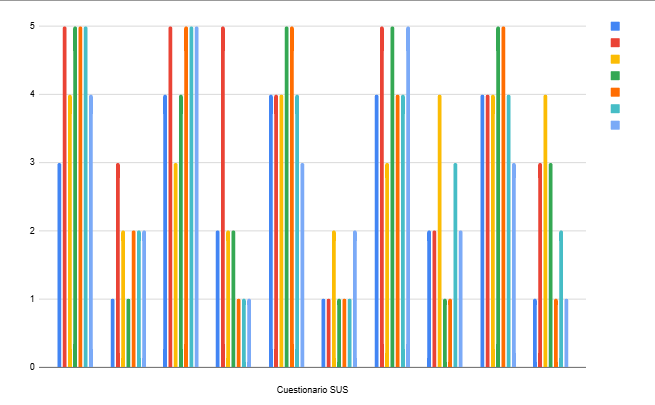
\includegraphics[height=5cm]{Imagenes/ResultadosSUS.png}
	\caption{Resultados obtenidos en el cuestionario SUS}
	\label{fig:Cuestionario SUS}
\end{figure}

A continuación se responderán las preguntas que se formularon previamente en la Sección~\ref{sec:preguntas}.


\subsubsection{Respuesta a la primera pregunta en la Sección~\ref{sec:intuitiva}}

\begin{enumerate}
    \item \textbf{¿El usuario entiende fácilmente cómo añadir funcionalidad al enemigo?} \\

Los ítems 3 (\textit{Pensé que el sistema era fácil de usar}) y 7 (\textit{Imaginaría que la mayoría de la gente aprendería a usar este sistema muy rápidamente}) reflejan como en ambos casos, más del 85\% de los usuarios se ubicaron en los valores altos de la escala (4 o 5), lo que indica que la adición de funcionalidades fue percibida como accesible e intuitiva. 

    \item \textbf{¿Las opciones de comportamiento ofrecidas son comprendidas en su totalidad?} \\

El ítem 6 (\textit{Pensé que había demasiada inconsistencia en este sistema}) arrojó valores predominantemente bajos (71,4\,\% marcó 1), lo que sugiere que los actuadores y comportamientos ofrecidos son coherentes entre sí y comprensibles. En la observación encontramos que ninguno usó los Tooltips creados que podrían haber servido para mejorar la comprensión fueron leídos, hablando con ellos se concluye que no sabían  que existían. Una posible mejora sería mencionarlos en el manual, ya que modificarlos visualmente podría sobrecargar la herramienta.

    \item \textbf{¿La interfaz comunica correctamente el propósito de cada estado y transición?} \\

El ítem 5 (\textit{Encontré que las diversas funciones de este sistema estaban bien integradas}) fue valorado positivamente por el 85,9\,\% de los usuarios (respuestas 4 y 5), lo que indica que la interfaz fue eficaz comunicando la relación entre los elementos de diseño (estados, transiciones, actuadores).

    \item \textbf{¿La documentación aclara y detalla la configuración de las funcionalidades?} \\

Aunque el cuestionario SUS no aborda directamente la calidad de la documentación, las respuestas cualitativas recogidas en las entrevistas reflejaron una valoración favorable en cuanto a la claridad del manual proporcionado, sin embargo destacaron que era muy largo. 
\end{enumerate}

\subsubsection{Respuestas a la segunda pregunta en la Sección~\ref{sec:funcional}}

\begin{enumerate}
    \item \textbf{¿La herramienta agiliza y simplifica el proceso de diseño de enemigos?} \\

Este aspecto se refleja indirectamente en los ítems 1 (\textit{Creo que me gustaría usar este sistema con frecuencia}) y 3 (\textit{Pensé que el sistema era fácil de usar}). La alta valoración obtenida (ambos con mayoría en los valores 4 y 5) respalda que los usuarios perciben la herramienta como útil y eficiente en su propósito de simplificar el diseño de enemigos.

    \item \textbf{¿El comportamiento de los enemigos generados se corresponde con lo esperado en el videojuego?} \\

En la observación realizada durante las pruebas encontramos que aunque si que hacían lo que los ejemplos del manual indicaban, les costaba comprenderlo. En la puesta en común se propuso la realización de videos donde se explicase de manera visual como se configuraba cada enemigo.

    \item \textbf{¿La herramienta permite la adaptación y expansión sencilla de los enemigos?} \\

El ítem 10 (\textit{Necesité aprender muchas cosas antes de poder usar este sistema}) proporciona una visión indirecta sobre la complejidad percibida. Aquí, la mayoría de usuarios marcó valores bajos (1 o 2), lo cual indica que la curva de aprendizaje no fue elevada y que la adaptación del sistema no requirió una sobrecarga cognitiva. Además, las entrevistas revelaron que los usuarios valoraron positivamente la modularidad de la herramienta.
\end{enumerate}
\subsubsection{Puesta en común}
Tras la realización del cuestionario se procedió a hacer una puesta en común con los usuarios. De ellas podemos sacar en claro que :
\begin{itemize}
\item Les ha gustado que la herramienta tenga tantos tipos de comportamientos y la ven muy completa.
\item No sabían de la existencia de Tooltips.
\item Les parece extraño tener que usar la pestaña de Animator y recomiendan su gestión desde el inspector.
\item Les gustaría tener video tutoriales donde se explique cada cosa de manera más visual.
\item Creen que tanto pinchar y arrastrar puede liar cuando hay muchos movimientos, lo que indica que estaría bien cambiar la forma en la que se visualizan los elementos para verla más clara y no uno tras otro sin saber que elementos están conectados con cuales.
\item Confusión general con estado de la Maquina de estados finita y estado de animación
\item Uno menciona la necesidad de más elementos de debug de forma visual
\item Necesario el feedback de daño en el jugador para verificar que los enemigos hacen daño
\end{itemize}
\subsection{Conclusión general}

La evaluación preliminar de la herramienta, realizada con un grupo limitado de solo siete participantes, sugiere que la usabilidad es generalmente aceptable en su versión actual. Se perciben fortalezas en la claridad de la interfaz, la integración de funcionalidades y una baja percepción de complejidad. Sin embargo, es importante señalar que la muestra reducida de usuarios impide que estos datos sean estadísticamente significativos o generalizables.\\

Las observaciones y respuestas cualitativas de este pequeño grupo indican posibles áreas de mejora en la herramienta. A pesar de estas sugerencias, parece cumplir los objetivos definidos a un nivel básico para los usuarios que la han probado.

